\section{Research Questions}
Our research questions aim to discover how people in the West, specifically, perceive armed conflicts. The way people perceive armed conflicts is at least partially a reflection of Western news cycles, and the way they talk about them is a reflection of their perception. However, which features of the conflicts cause these perceptions in the first place? Are they the same features that have been linked to news reporting?

Our data set consists of approximately two terabytes of Reddit data, ranging from the year 2012 to the year 2014. These comments span every subreddit. Reddit, being a large, mostly Western community with somewhat homogeneous viewpoints (compared to other data sources like Twitter) gives an interesting outlet to answer such questions. Over a large dataset, we will focus on asking simple questions with clear answers and then using those answers to integrate with what's already been studied about social phenomena such as news cycles and network effects of news distribution. We will then cross-reference this with data on armed conflicts from the Armed Conflict Database. 

\begin{figure}
\centering
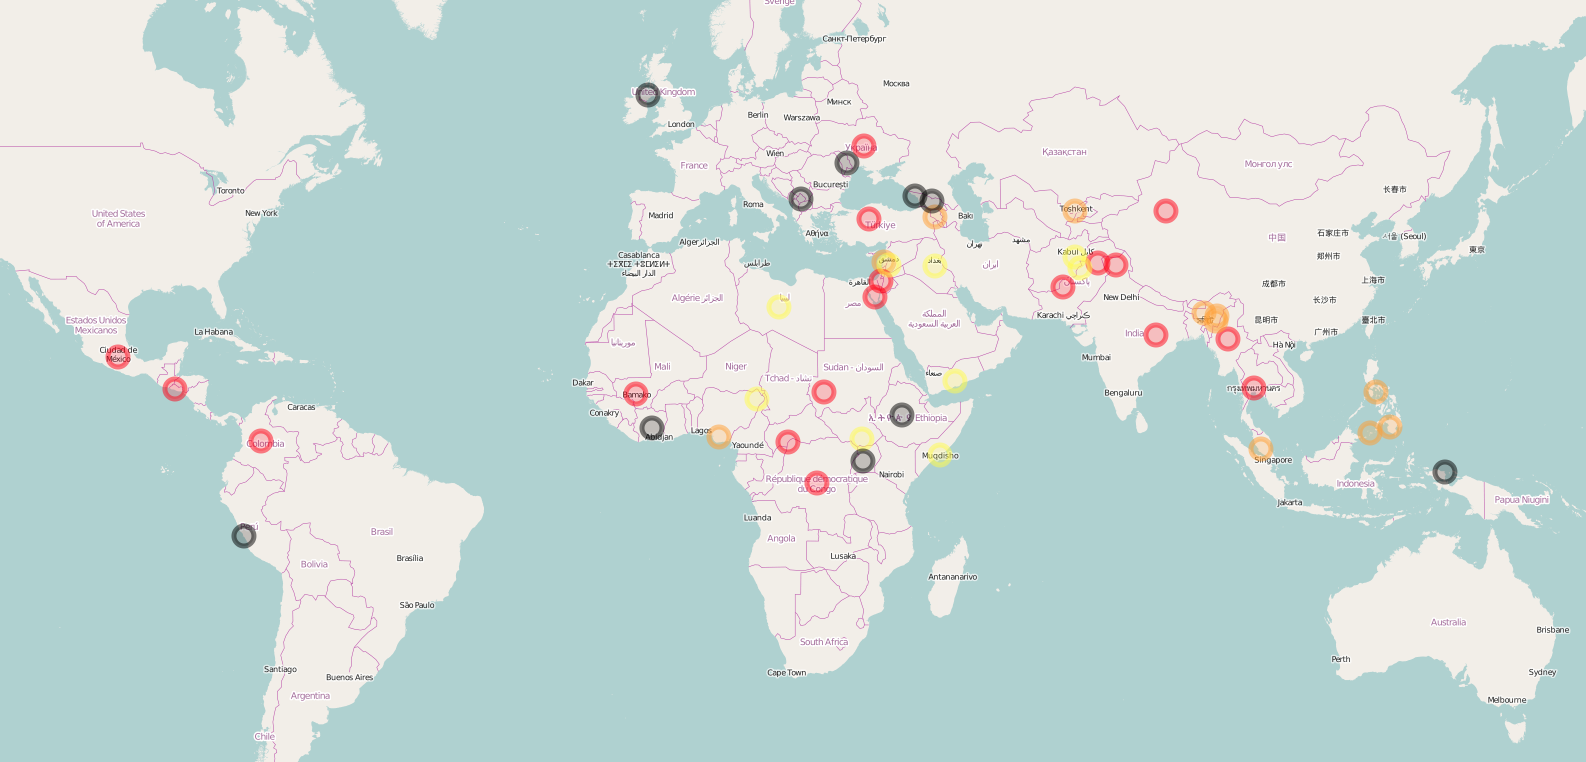
\includegraphics[width=0.9\columnwidth]{map}
\caption{A map of 48 conflicts. Black, yellow, orange and red circles indicate the current level of intensity as rated by the Armed Conflict Database: archived, low, medium and high, respectively.}
\label{conflicts}
\end{figure}

To ensure that none of the conflicts are considered purely historical, we chose 48 conflicts that had nonzero fatalities in at least one of the years between 2012 and 2014. See Figure~\ref{conflicts} for a summary of where the conflicts occurred. 

Thus, there are two main features of the comments we find interesting. The first is the \textit{sentiment}. Using the sentiment analyzer bundled with StanfordNLP\cite{stanfordnlp}, we rated over 25,000 comments as Very Negative, Negative, Neutral, Positive, or Very Positive. The second is the \textit{acceptability}. The acceptability references how the community perceives the comment, and thus that sentiment. 

From our exploratory data analysis, sentiment did not appear to be correlated with acceptability. We decided this meant that it was better to ask questions of negative sentiment and positive sentiment individually. We wanted to examine several factors that could affect news reports discussing the conflict, with the thought that they might also influence how they are discussed on social media.

\begin{enumerate}
\item{\textbf{Severity.} This includes the total number of people who were killed, made refugees, or internally displaced as a result of the conflict. While common sense would suggest that severity should play a large role in perception, previous work suggests that it doesn't play as large of one as one might think.} 
\item {\textbf{Location.} There are six major regions that the Armed Conflict Database groups conflicts into. We hypothesize that regions that share more cultural similarity would be viewed differently than regions which share less.} 
\item {\textbf{Recent (or marginal) Severity.} This includes the number of people who were killed, made refugees, or internally displaced the same year the comment was made. In other words, do recent fatalities salience cause them to be treated differently than former fatalities? From previous research, we suspected that marginal severity would play a larger role than total severity.}
\item {\textbf{Age.} The number of years ago the conflict started. We hypothesized Age would be a significant correlate due to waning interest. After decades of conflict, it is perhaps difficult for some users to still empathize with any tragedy.}
\item {\textbf{Nature.} What characterizes the conflict? Why did it start? These include Separatism, Terrorism, Foreign Antagonism, Disputes over Territory, Criminal Activity, and Ethnic Violence. We hypothesized that those that are easier for Westerners to empathize with due to history, such as Separatism or Foreign Antagonism, might be treated differently than those whose common perception is that it is the type of conflict that only uncivilized nation-states engage in.}
\item {\textbf{Expert Perception.} The Armed Conflict Database rates conflicts for their current level of intensity. While this is obviously correlated with deaths, refugees, and IDP ($p < 0.0001$), the average person may be more likely to get their ideas of severity from experts, rather than numbers. It is also unclear how well the perception of the Armed Conflict Database would correlate with the perception of traditional media, which is a more likely source ofor information.} 
\end{enumerate}